\section{Kiến trúc triển khai (Deployment View)}
\begin{figure}[H]
	\centering
	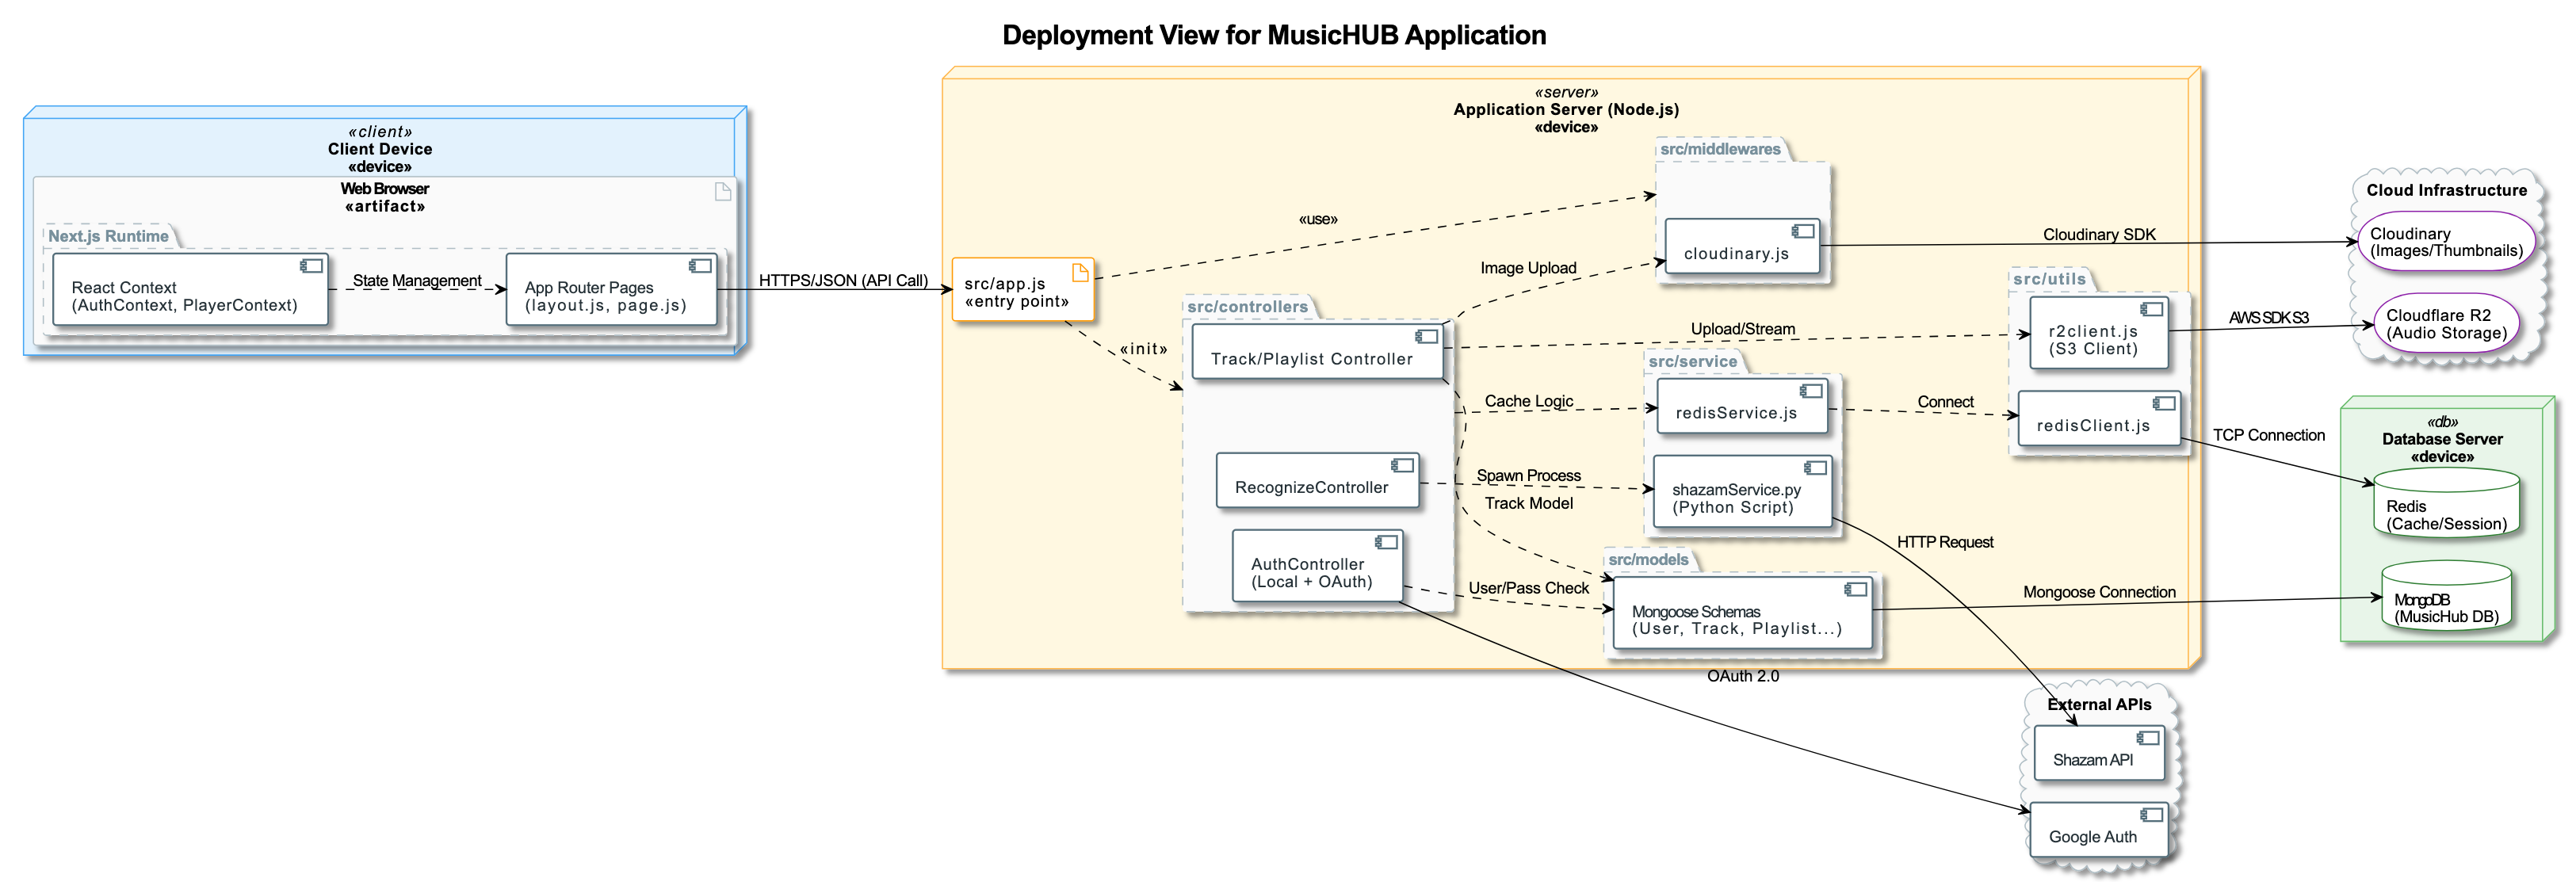
\includegraphics[width=\textwidth]{Images/deployment.png}
	\caption{Deployment View của hệ thống}
\end{figure}

\subsection{Tổng quan}
Deployment View (Sơ đồ triển khai) mô tả kiến trúc vật lý của hệ thống MusicHUB, minh họa cách các thành phần phần mềm (Software Artifacts) được phân bố trên các node phần cứng hoặc môi trường ảo hóa. Sơ đồ thể hiện sự tương tác giữa Client, Application Server, Database Server và các dịch vụ Cloud bên thứ ba. \\ \\
Để tăng tính trực quan, các thành phần trong sơ đồ được phân loại theo nhóm chức năng:
\begin{itemize}
    \item \textbf{Client Tier (Màu xanh dương):} Giao diện tương tác người dùng.
    \item \textbf{Application Tier (Màu vàng):} Trung tâm xử lý logic nghiệp vụ.
    \item \textbf{Data Tier (Màu xanh lá):} Lưu trữ và quản lý dữ liệu.
    \item \textbf{Cloud \& External (Màu xám):} Hạ tầng mạng và dịch vụ tích hợp.
\end{itemize}

\subsection{Chi tiết các thành phần}
\subsubsection{Client Tier (Tầng Khách hàng)}
Môi trường tương tác trực tiếp với người dùng cuối:
\begin{itemize}
    \item \textbf{Thiết bị:} Web Browser (Trình duyệt web).
    \item \textbf{Artifacts:}
    \begin{itemize}
        \item \textbf{Next.js Runtime:} Chạy ứng dụng Frontend (React 19) với Server-side Rendering.
        \item \textbf{App Router Pages:} Hệ thống routing hiện đại của Next.js (\texttt{layout.js}, \texttt{page.js}).
        \item \textbf{State Management:} Sử dụng React Context (\texttt{AuthContext}) để quản lý phiên đăng nhập cho cả hai phương thức (Local \& OAuth).
    \end{itemize}
    \item \textbf{Giao thức:} Giao tiếp qua HTTPS/JSON API.
\end{itemize}

\subsubsection{Application Tier (Tầng Ứng dụng)}
Đóng vai trò trung tâm xử lý nghiệp vụ, được triển khai trên môi trường \textbf{Node.js Server}.
\begin{itemize}
    \item \textbf{Entry Point (\texttt{src/app.js}):} Điểm khởi chạy ứng dụng.
    \item \textbf{Controllers (\texttt{src/controllers}):} 
    \begin{itemize}
        \item \texttt{AuthController}: Quản lý hệ thống xác thực kép (Dual Authentication System):
        \begin{itemize}
            \item Xác thực truyền thống: Email/Password kết hợp mã hóa Bcrypt.
            \item Xác thực xã hội: Google OAuth 2.0.
        \end{itemize}
        \item \texttt{Track/Playlist Controller}: Quản lý streaming và danh sách phát.
        \item \texttt{RecognizeController}: Xử lý nhận diện nhạc.
    \end{itemize}
    \item \textbf{Integration Services:}
    \begin{itemize}
        \item \textbf{Shazam Service:} Script Python (\texttt{shazamService.py}) để giao tiếp với Shazam API.
        \item \textbf{Cloud Clients:} Các module kết nối Cloudflare R2 và Redis.
    \end{itemize}
\end{itemize}

\subsubsection{Data Tier (Tầng Dữ liệu)}
\begin{itemize}
    \item \textbf{MongoDB (Primary Database):} 
    \begin{itemize}
        \item Lưu trữ thông tin người dùng bao gồm mật khẩu đã mã hóa (Hashed Password) và thông tin Profile từ Google.
        \item Sử dụng Mongoose Schemas để định nghĩa cấu trúc dữ liệu.
    \end{itemize}
    \item \textbf{Redis (Cache \& Session):} Lưu trữ Session đăng nhập (JWT Whitelist/Blacklist) để tối ưu hiệu năng xác thực.
\end{itemize}

\subsection{Các luồng dữ liệu chính (Data Flows)}

\subsubsection{Quy trình Xác thực (Authentication Flow)}
Hệ thống hỗ trợ hai luồng đăng nhập song song:
\begin{enumerate}
    \item \textbf{Đăng nhập truyền thống (Traditional Login):} Client $\rightarrow$ \texttt{AuthController} $\rightarrow$ Kiểm tra Email $\rightarrow$ So khớp Bcrypt Hash $\rightarrow$ Tạo JWT Token $\rightarrow$ Lưu Session vào Redis.
    \item \textbf{Đăng nhập qua Google (OAuth Login):} Client $\rightarrow$ \texttt{AuthController} $\rightarrow$ Redirect Google OAuth $\rightarrow$ Lấy Profile Data $\rightarrow$ Tạo/Cập nhật User $\rightarrow$ Tạo JWT Token $\rightarrow$ Lưu Session vào Redis.
\end{enumerate}

\subsubsection{Các luồng nghiệp vụ khác}
\begin{enumerate}
    \item \textbf{Upload nhạc:} Client $\rightarrow$ Middleware Upload $\rightarrow$ Cloudinary (Ảnh) + R2 (Audio) $\rightarrow$ Lưu Metadata vào MongoDB.
    \item \textbf{Streaming Nhạc:} Client $\rightarrow$ \texttt{TrackController} $\rightarrow$ Lấy URL từ Cloudflare R2 $\rightarrow$ Stream về Client.
    \item \textbf{Nhận diện nhạc:} Client $\rightarrow$ \texttt{RecognizeController} $\rightarrow$ \texttt{shazamService.py} $\rightarrow$ Shazam API.
\end{enumerate}

\subsection{Đặc điểm kỹ thuật \& Bảo mật}
\begin{itemize}
    \item \textbf{Password Security:} Mật khẩu người dùng không bao giờ được lưu dưới dạng văn bản thuần (plain text). Hệ thống sử dụng thư viện \textbf{Bcrypt} để băm (hash) mật khẩu trước khi lưu vào MongoDB.
    \item \textbf{Stateless Authentication:} Sử dụng \textbf{JWT (JSON Web Token)} để quản lý phiên làm việc, cho phép xác thực không trạng thái và dễ dàng mở rộng (scale).
    \item \textbf{Secure Communication:} Toàn bộ giao tiếp giữa Client và Server được mã hóa qua giao thức HTTPS/TLS.
    \item \textbf{Environment Security:} Các thông tin nhạy cảm (JWT Secret, Database URI, API Keys) được quản lý chặt chẽ qua biến môi trường.
\end{itemize}